\documentclass[11pt,letterpaper]{article}
\usepackage[margin=2cm]{geometry}
\usepackage{amsmath,amssymb,graphicx,xcolor,booktabs,tabularx,enumitem,titlesec,fancyhdr,array,longtable}
\usepackage{tikz}
\usetikzlibrary{arrows.meta,positioning,shapes.geometric,fit,calc,decorations.pathreplacing}
\usepackage[hidelinks]{hyperref}
\usepackage{helvet}\renewcommand{\familydefault}{\sfdefault}
\usepackage{caption}
\titleformat{\section}{\Large\bfseries\color{blue!50!black}}{\thesection}{0.6em}{}
\titleformat{\subsection}{\large\bfseries}{\thesubsection}{0.6em}{}
\titleformat{\subsubsection}{\normalsize\bfseries}{\thesubsubsection}{0.6em}{}
\setlength{\headheight}{14pt}
\setlist{itemsep=1pt,topsep=3pt}
\setlength{\emergencystretch}{3em}
\setlength{\parskip}{3pt}
\newcommand{\boxit}[4]{\par\medskip\noindent\fcolorbox{#1}{#2}{\begin{minipage}{0.955\linewidth}\textbf{#3}\par\smallskip #4\end{minipage}}\par\medskip}
\newcommand{\conceptbox}[2]{\boxit{blue!50!black}{blue!4}{#1}{#2}}
\newcommand{\connectbox}[1]{\boxit{green!40!black}{green!5}{Connect to your analysis}{#1}}
\newcommand{\pitfallbox}[1]{\boxit{red!60!black}{red!4}{Pitfalls}{#1}}
\newcommand{\checksbox}[1]{\boxit{orange!70!black}{orange!6}{Checks}{#1}}
\newcommand{\goal}[1]{\par\noindent\textbf{Goal.} #1\par}
\newcommand{\exbox}[2]{\boxit{gray!60!black}{gray!6}{Optional exercise #1}{#2}}
\pagestyle{fancy}\fancyhf{}\lhead{sPHENIX Self-Paced Course}\rhead{Module 8: Tracking Reconstruction}\cfoot{\thepage}
\begin{document}
\begin{center}
{\LARGE\bfseries sPHENIX Self-Paced Course --- Module 8:}\\[4pt]
{\Large\bfseries Tracking reconstruction: seeding, fitting, alignment and TPC calibration}\\[8pt]
November 2026 \quad Prepared for P.\,D.\ Lewis (Ohio University)\\[2pt]
\small Self-contained study text based on the Summer-2026 sPHENIX School, public sPHENIX documents and standard textbook material
\end{center}

\tableofcontents
\newpage

\section*{How to use this module}
\addcontentsline{toc}{section}{How to use this module}
This module is self-contained. It starts from the physics of a charged particle in a magnetic field and ends with the
calibrations and performance checks that decide whether sPHENIX tracks are good enough for physics.
The school talks below are the sources; you do not need them to follow the text.
Tracking is the part of the experiment furthest from your own analysis, so the text explains each idea from scratch and points out where it touches calorimeter work.

\subsection*{Learning objectives}
\begin{enumerate}[label=O\arabic*.]
\item Derive the momentum resolution of a tracker from measurement error and multiple scattering, and apply it to sPHENIX numbers.
\item Describe the sPHENIX tracking workflow from raw streaming data to fitted tracks, including why a Fun4All ``event'' is not a physics event.
\item Explain silicon triplet seeding, TPC cellular-automaton seeding and silicon--TPC matching.
\item Explain the Kalman filter (prediction, update, smoothing) and how ACTS is used for the final fit and vertexing.
\item Explain track-based alignment with Millepede, including local versus global parameters and weak modes.
\item Explain TPC distortions (static, average, event-by-event), their physics origin, and the calibration tools: drift velocity, lasers, central membrane, track residuals, digital currents, gain.
\item Explain track--calorimeter matching and how it serves electron identification, momentum scale and calorimeter checks.
\item Name the performance metrics (efficiency, fake rate, momentum resolution, DCA resolution, residuals) and how each is measured.
\end{enumerate}

\subsection*{Prerequisites}
Module 4 (tracking detectors), Module 6 (Fun4All, node tree, DSTs). Basic linear algebra (matrices, least squares).

\subsection*{Estimated time}
About 9--11 hours of reading; 3 hours for the optional exercises.

\subsection*{Sources (school talks, sPHENIX School 2026)}
\begin{itemize}
\item {[S19]} J.~Osborn, ``Tracking Reconstruction''.
\item {[S20]} G.~Ottino, ``Tracking Alignment''.
\item {[S22]} M.~Mitrankova, ``TPC Calibration''.
\item {[S23]} X.~Yu, ``Track-Calo Matching''.
\item {[S36]} A.~P.~Dash, ``Tracking Performance Evaluation in sPHENIX (flash)''.
\item {[S27]} A.~Patton, ``Machine Learning Momentum Scale Correction (flash)''.
\end{itemize}

\subsection*{Public readings (optional)}
ACTS [R1]; Kalman filtering for tracks [R2]; Millepede [R3]; Gluckstern's resolution formulae [R4]; the sPHENIX proposal [R5]; INTT papers [R6, R7].

\conceptbox{Conventions}{sPHENIX code uses centimetres; ACTS uses millimetres internally [S20]. Momenta in GeV/$c$, fields in tesla.
``Toy'' marks illustrative numbers of my own. Detector dimensions are public design values and are quoted approximately.}

%=====================================================================
\section{Tracking primer: what limits a momentum measurement}
%=====================================================================
\goal{Derive the two terms of the momentum resolution and see how sPHENIX's design balances them.}

\subsection{Helix and sagitta}
In a uniform field $B$ along $z$, a particle of charge $q=\pm e$ moves on a helix. Its projection on the transverse plane is a circle of radius
\begin{equation}
R\,[\mathrm{m}] = \frac{p_T\,[\mathrm{GeV}/c]}{0.3\,B\,[\mathrm{T}]}.
\end{equation}
Over a chord of length $L$ the deviation from a straight line, the \emph{sagitta}, is $s\approx L^2/(8R)$.
\textbf{Worked example.} The TPC spans radii of roughly 20 to 78~cm [R5], so $L\approx0.58$~m. In $B=1.4$~T:
for $p_T=1$~GeV/$c$, $R=2.38$~m and $s=0.58^2/(8\times2.38)\approx1.8$~cm; for $p_T=10$~GeV/$c$, $s\approx1.8$~mm.
A position resolution of order 100~$\mu$m per point is therefore a small fraction of the sagitta at 1~GeV/$c$ but a larger fraction at 10~GeV/$c$.

\subsection{Measurement term}
For $N$ equally spaced points of resolution $\sigma_x$ over length $L$, Gluckstern's result [R4] is
\begin{equation}
\left(\frac{\sigma_{p_T}}{p_T}\right)_{\mathrm{meas}} = \frac{\sigma_x\,p_T}{0.3\,B\,L^2}\sqrt{\frac{720}{N+4}} .
\end{equation}
It grows linearly with $p_T$ (stiffer tracks have smaller sagitta) and falls as $1/(BL^2)$, which is why a strong field and a long lever arm matter most [S19].
\textbf{Worked example (toy point resolution).} With $N=48$ TPC layers, $\sigma_x=150~\mu$m, $L=0.58$~m, $B=1.4$~T and $p_T=1$~GeV/$c$:
$\sigma/p_T\approx(1.5\times10^{-4})/(0.42\times0.336)\times\sqrt{720/52}\approx0.4\%$; at 10~GeV/$c$ it is $\approx4\%$.
Adding precise silicon points at small radius lengthens the effective lever arm and improves this.

\subsection{Multiple-scattering term}
A charged particle crossing material of thickness $x$ is deflected by many small Coulomb scatterings. The projected angular spread is given by the standard Highland formula
\begin{equation}
\theta_0 = \frac{13.6~\mathrm{MeV}}{\beta c p}\,|z|\sqrt{\frac{x}{X_0}}\left[1+0.038\ln\frac{x}{X_0}\right].
\end{equation}
Because $\theta_0\propto1/p$ and the bending also scales as $1/p$, the resulting momentum error is independent of $p$ (for $\beta\approx1$):
\begin{equation}
\left(\frac{\sigma_{p_T}}{p_T}\right)_{\mathrm{MS}} \approx \frac{0.0136}{0.3\,\beta\,B\,L}\sqrt{\frac{L}{X_0}}\times C, \qquad C\approx1.3\text{--}1.4.
\end{equation}
The total resolution is the quadrature sum: a constant multiple-scattering floor at low $p_T$ and a term rising linearly at high $p_T$ [S19].
This explains the design rules: thin material (gas in the TPC, thin silicon), large $B$, long $L$, many points.

\subsection{Pointing resolution}
For heavy flavour, what matters is the distance of closest approach (DCA) of a track to the primary vertex. Charm hadrons fly about 50--300~$\mu$m before decaying [S20], so the DCA resolution must be a few tens of micrometres.
\textbf{Worked example.} A silicon layer of about 0.3\% $X_0$ (a typical thin MAPS layer) at a radius of about 2.5~cm: for $p=1$~GeV/$c$,
$\theta_0\approx13.6\times10^{-3}\times\sqrt{0.003}\times(1+0.038\ln0.003)\approx0.6$~mrad, which displaces the extrapolated track by $\approx0.6\times10^{-3}\times25$~mm $\approx15~\mu$m.
Multiple scattering in the beam pipe and the first layer, and the intrinsic resolution of the innermost layers, set the DCA resolution at low $p_T$.
This is also why alignment of the innermost silicon to a few micrometres is essential (Section~\ref{sec:align}).

%=====================================================================
\section{The detectors as seen by reconstruction}
%=====================================================================
\goal{Recall what each tracker contributes, with emphasis on timing.}

\begin{figure}[h]\centering
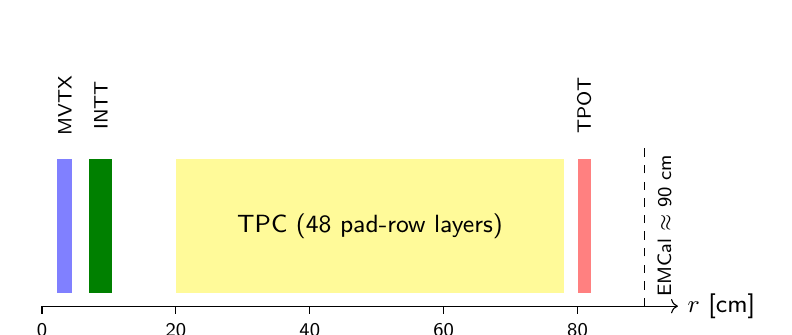
\begin{tikzpicture}[scale=0.085]
\draw[->] (0,0) -- (95,0) node[right,font=\small]{$r$ [cm]};
\foreach \r/\l in {0/0,20/20,40/40,60/60,80/80} { \draw (\r,0) -- (\r,-1.2); \node[below,font=\scriptsize] at (\r,-1.2) {\l}; }
\fill[blue!50] (2.3,2) rectangle (4.5,22); \node[font=\scriptsize, rotate=90] at (3.4,30) {MVTX};
\fill[green!50!black] (7,2) rectangle (10.5,22); \node[font=\scriptsize, rotate=90] at (8.8,30) {INTT};
\fill[yellow!40] (20,2) rectangle (78,22); \node[font=\small] at (49,12) {TPC (48 pad-row layers)};
\fill[red!50] (80,2) rectangle (82,22); \node[font=\scriptsize, rotate=90] at (81,30) {TPOT};
\draw[dashed] (90,0) -- (90,24); \node[font=\scriptsize, rotate=90] at (93,12) {EMCal $\approx$ 90 cm};
\end{tikzpicture}
\caption{Schematic radial layout of the tracking system (own drawing, approximate public design radii, not to scale in $z$).}\label{fig:layout}
\end{figure}

\begin{itemize}
\item \textbf{MVTX}: three layers of monolithic active pixel sensors at small radius. Very precise space points; the key to the DCA. Its integration (strobe) time spans several microseconds, i.e.\ many bunch crossings.
\item \textbf{INTT}: two layers of silicon strips. Its timing resolves the single bunch crossing, so it tags which crossing a track came from [R6, R7].
\item \textbf{TPC}: a gas time projection chamber from about 20 to 78~cm with 48 pad-row layers, read by GEMs [S22]. It measures $r\phi$ precisely; $z$ comes from the drift time, which is only meaningful once the collision time (crossing) is known. The full drift takes of order ten microseconds.
\item \textbf{TPOT}: micromegas modules just outside the TPC in a limited acceptance, giving precise points that anchor TPC calibration [S22].
\end{itemize}
The detectors run in streaming mode at least in part, with very different integration times.
This drives the whole reconstruction design.

\subsection{A Fun4All event is not a physics event}
Raw tracker data are streams of hits stamped with the beam-clock counter (BCO). The event combiner uses the GL1 trigger as reference and collects all hits within a \emph{trigger frame},
a fixed block of time around the trigger [S19]. In the reconstructed data the triggered crossing has the most seeds, but seeds from other crossings within the frame are present at a roughly flat rate [S19].
Hence one Fun4All ``event'' can contain several collisions from different crossings, and the reconstruction itself must assign tracks to crossings and vertices [S19].

\connectbox{For calorimeter-only analyses this subtlety is hidden: calorimeters are read out only for triggered crossings. As soon as you combine tracks with
calorimeter clusters, you must keep only tracks assigned to the triggered crossing (crossing zero) [S23]. Otherwise you will match clusters with tracks from a different collision.}

%=====================================================================
\section{The reconstruction workflow}\label{sec:workflow}
%=====================================================================
\goal{Know the jobs and DST levels of tracking production.}

\begin{figure}[h]\centering
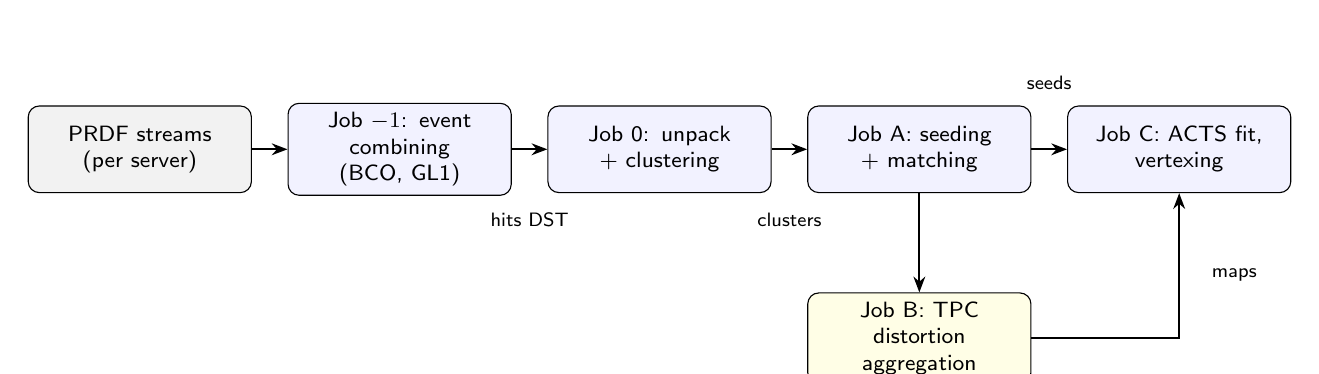
\begin{tikzpicture}[every node/.style={font=\footnotesize},
 box/.style={draw, rounded corners, text width=26mm, minimum height=11mm, align=center, fill=blue!5},
 arr/.style={-{Stealth[length=2mm]}, thick}]
\node[box, fill=gray!10] (raw) at (0,0) {PRDF streams\\(per server)};
\node[box] (j1) at (3.3,0) {Job $-1$: event\\combining (BCO, GL1)};
\node[box] (j0) at (6.6,0) {Job 0: unpack\\+ clustering};
\node[box] (ja) at (9.9,0) {Job A: seeding\\+ matching};
\node[box] (jc) at (13.2,0) {Job C: ACTS fit,\\vertexing};
\node[box, fill=yellow!10] (jb) at (9.9,-2.4) {Job B: TPC distortion\\aggregation};
\draw[arr] (raw) -- (j1); \draw[arr] (j1) -- (j0); \draw[arr] (j0) -- (ja); \draw[arr] (ja) -- (jc);
\draw[arr] (ja.south) -- (jb.north); \draw[arr] (jb.east) -| (jc.south);
\node[font=\scriptsize] at (4.95,-0.9) {hits DST}; \node[font=\scriptsize] at (8.25,-0.9) {clusters}; \node[font=\scriptsize] at (11.55,0.85) {seeds}; \node[font=\scriptsize] at (13.9,-1.6) {maps};
\end{tikzpicture}
\caption{Schematic tracking production chain (own drawing, simplified from [S19]).}\label{fig:wf}
\end{figure}

The chain [S19] is:
\begin{enumerate}
\item \textbf{Job $-1$, event combining.} Build trigger frames from the streams of every MVTX, INTT, TPC and TPOT server.
\item \textbf{Job 0, unpacking and clustering.} Convert hits to offline format and cluster them (Section~\ref{sec:clus}).
\item \textbf{Job A, pattern recognition.} Silicon seeding and TPC seeding run separately (their computational needs differ), then seeds are matched.
\item \textbf{Job B, distortion aggregation.} TPC residuals and central-membrane information from many files are aggregated into correction maps (Section~\ref{sec:tpccal}).
\item \textbf{Job C, fitting.} The ACTS track fit with alignment and distortion corrections applied to clusters on the fly, ghost removal, vertex finding and propagation to the vertex.
\end{enumerate}
The DST levels you can start from are, from lowest to highest, raw hits (\texttt{DST\_STREAMING\_EVENT}), clusters (\texttt{DST\_TRKR\_CLUSTER}), seeds (\texttt{DST\_TRKR\_SEED}) and tracks (\texttt{DST\_TRKR\_TRACKS}) [S23].
Start as high as your study allows: re-running seeding is expensive.

\conceptbox{Design principle: calibrate late}{Seeding is the most CPU-intensive step, so it cannot be rerun often. Calibrations (alignment, distortion corrections) are therefore applied as late as possible:
to clusters, on the fly, during the final fit [S19]. A new alignment or distortion map then requires only a refit from seeds, not a new seeding pass.}

\subsection{Why CPU and disk dominate the design}
The tracking volume of a heavy-ion run is many petabytes, and reconstruction takes several CPU-seconds per event.
Multiplying the two shows that a full pass over a large Au+Au dataset occupies the whole farm for months, and that data must be staged from tape at a limited rate [S19].
Consequences: production passes are planned carefully, intermediate DSTs cannot all be kept, and analysis-level shortcuts (lighter DSTs, compressed outputs) are actively developed [S19].

%=====================================================================
\section{Clustering}\label{sec:clus}
%=====================================================================
\goal{Understand how hits become space points with uncertainties.}

\subsection{Why clusters}
A particle usually fires more than one readout element: charge diffuses and is shared between neighbouring pixels, strips or pads.
Clustering groups these hits and computes a centroid, which is more precise than any single element [S19].
Every hit and cluster is labelled with a \emph{hitset key}, which identifies a detector surface uniquely; clusters live in a \texttt{TrkrClusterContainer} [S19].

\subsection{By detector}
\begin{itemize}
\item \textbf{MVTX} (\texttt{MvtxClusterizer}): binary pixels, so the centroid is a geometric average; cluster size depends on incidence angle and charge sharing.
\item \textbf{INTT} (\texttt{InttClusterizer}): strips with coarse ADC, plus the crossing (time) information that is later used to tag the collision.
\item \textbf{TPC} (\texttt{TpcClusterizer}, followed by \texttt{TpcClusterCleaner}): two-dimensional clusters in pad and time bin on each pad row; the centroid is ADC-weighted. Laser events are identified separately (\texttt{LaserEventIdentifier}) so that they do not enter physics tracking.
\item \textbf{TPOT} (\texttt{MicromegasClusterizer}): strips in one coordinate per module.
\end{itemize}
The unpackers in the public macros are \texttt{MvtxCombinedRawDataDecoder}, \texttt{InttCombinedRawDataDecoder}, \texttt{TpcCombinedRawDataUnpacker} and \texttt{MicromegasCombinedDataDecoder}.

\subsection{Differential nonlinearity}
With shaped (zig-zag) pads, the ADC-weighted centroid is not a linear function of the true position across the pad: it is pulled towards certain positions.
This differential nonlinearity can be measured in simulation by comparing the cluster centroid with the true crossing point of the Geant4 track at the layer radius, and then corrected [S22].
\emph{Analogy:} it is the tracker version of the EMCal centre-of-gravity S-curve (Module 7).

\pitfallbox{\begin{itemize}
\item A hot channel creates fake clusters in every frame; a dead region removes points. Both must be in the simulation (hot/dead maps) for efficiency estimates [S19].
\item TPC cluster $z$ is not known at clustering time: it is a drift time until the crossing is assigned.
\end{itemize}}
%=====================================================================
\section{Seeding and track finding}
%=====================================================================
\goal{Understand how initial track candidates are found among $O(10^5)$ clusters.}

\subsection{The combinatorial problem}
With one track, picking its clusters is trivial. In a central heavy-ion event there are thousands of particles and of order $10^5$ clusters, plus noise and out-of-time hits [S19].
Naively testing every pair or triplet of clusters scales as $N^2$ or $N^3$; the cost of later stages scales with the number of seeds [S19].
Good seeding must therefore be efficient (find real tracks), pure (few fakes) and fast.
Track reconstruction is split into three stages [S19]: \emph{seeding} (an initial guess from a few points), \emph{finding} (adding further clusters along the predicted path) and \emph{fitting} (precise parameters).

\subsection{Silicon seeding}
Silicon seeds are found with the ACTS triplet seeder, wrapped in \texttt{PHActsSiliconSeeding} [S19]:
\begin{enumerate}
\item \textbf{Pass 1}: form triplets in the three MVTX layers (a circle through three points gives curvature and direction), then project to the INTT to attach matching clusters.
\item \textbf{Pass 2}: form triplets using MVTX and INTT together, and project to layers missing from the triplet.
\end{enumerate}
Seeding is ``4D'': clusters must match in space \emph{and} in time [S19]. The INTT timing assigns the bunch crossing; the MVTX integration window must contain it.
Duplicates from the two passes are merged (\texttt{PHSiliconSeedMerger}).
The seeding acceptance is reproduced in simulation once the survey geometry and hot/dead maps are included [S19].

\conceptbox{Why triplets?}{Three points determine a circle in the transverse plane (curvature, direction, impact parameter) and a line in $r$--$z$.
Cuts on the implied $p_T$, the compatibility with the beam line and the consistency of the three points reject most random combinations before any expensive fit.}

\subsection{TPC seeding: the cellular automaton}
In the TPC, a track leaves a long chain of points on consecutive pad rows. The cellular-automaton (CA) seeder, \texttt{PHCASeeding}, exploits this [S19]:
\begin{enumerate}
\item For each cluster, find candidate neighbours on adjacent layers within a window.
\item Keep links that are \emph{mutual}: cluster $a$ points to $b$ as its best continuation and $b$ points back to $a$. This builds a directed graph of short segments.
\item Follow the chains of links to build seeds that span many layers.
\item Extend each seed with a Kalman-filter propagator (\texttt{PHSimpleKFProp}) that adds clusters compatible with the predicted path.
\end{enumerate}
The method is based on the ALICE TPC seeding, which runs on GPUs; the sPHENIX implementation runs on CPUs [S19].
An alternative seeder working in local TPC coordinates with a zeroth-order distortion correction was being compared [S19].
Before matching, TPC seeds are moved to point to $z=0$, given preliminary distortion corrections (\texttt{PrelimDistortionCorrection}), refitted and moved back [S19].

\subsection{Matching silicon and TPC seeds}
Silicon and TPC seeds are matched in $\eta$, $\phi$ and the position of closest approach $(x,y,z)$ (\texttt{PHSiliconTpcTrackMatching}) [S19].
The $z$ matching is subtle: the TPC measures drift time, not $z$. Only after matching to a silicon seed, whose crossing is known from the INTT, can the TPC clusters be placed in $z$ [S19].
The crossing number is applied to the TPC seed; then matched seeds are extended to TPOT (\texttt{PHMicromegasTpcTrackMatching}) and passed to the fitter.

\textbf{Worked example (toy numbers).} With an electron drift velocity of about 8~cm/$\mu$s, an error of one bunch crossing ($\approx$106~ns) in the assumed collision time shifts every TPC cluster by $\approx0.85$~cm in $z$.
Without the INTT crossing tag, the TPC alone cannot locate tracks in $z$ to better than this.

%=====================================================================
\section{Track fitting with the Kalman filter}
%=====================================================================
\goal{Understand the Kalman filter well enough to read residual plots and fit outputs.}

\subsection{The idea}
A Kalman filter estimates a state that evolves deterministically (here: the track parameters along the trajectory) from a sequence of noisy measurements [S19, R2].
It alternates two steps: \emph{predict} the state at the next measurement surface, then \emph{update} the prediction with the measurement, weighting each by its uncertainty.
Its advantages over a global fit are that it handles multiple scattering and energy loss naturally (as process noise) and that it can add or reject hits as it goes.

\subsection{The equations}
Let $\mathbf{x}_k$ be the track state at surface $k$ (for example two local positions, two angles and $q/p$) with covariance $C_k$.
\begin{itemize}
\item \textbf{Prediction.} Propagate through the field: $\mathbf{x}_{k|k-1}=f(\mathbf{x}_{k-1})$, with Jacobian $F_k$ and process noise $Q_k$ from multiple scattering:
\begin{equation}
C_{k|k-1} = F_k\,C_{k-1}\,F_k^{T} + Q_k .
\end{equation}
\item \textbf{Update.} With measurement $\mathbf{m}_k$, projection matrix $H_k$ and measurement covariance $V_k$:
\begin{align}
K_k &= C_{k|k-1}H_k^T\left(V_k + H_kC_{k|k-1}H_k^T\right)^{-1},\\
\mathbf{x}_k &= \mathbf{x}_{k|k-1} + K_k\left(\mathbf{m}_k - H_k\mathbf{x}_{k|k-1}\right),\qquad C_k=(1-K_kH_k)\,C_{k|k-1}.
\end{align}
The residual $\mathbf{r}_k=\mathbf{m}_k-H_k\mathbf{x}_{k|k-1}$ and its covariance give a $\chi^2$ increment, used to reject outliers.
\item \textbf{Smoothing.} After the last measurement, a backward pass combines all information so that every surface has the best estimate (``smoothed states'') [S19].
\end{itemize}

\subsection{A one-dimensional toy}
Estimate a constant $x$ from measurements with error $\sigma$. Start with a vague prior ($C_0\to\infty$).
After the first measurement $K_1=1$, so $x_1=m_1$, $C_1=\sigma^2$. After the second, $K_2=C_1/(\sigma^2+C_1)=\tfrac12$, so $x_2=(m_1+m_2)/2$ and $C_2=\sigma^2/2$.
After $n$ steps $x_n$ is the mean and $C_n=\sigma^2/n$: the filter reproduces least squares. With process noise $Q>0$ (a ``wandering'' state, like a scattered track) older measurements are progressively down-weighted.

\subsection{ACTS in sPHENIX}
ACTS [R1] is an experiment-independent tracking toolkit derived from ATLAS software. sPHENIX uses it for geometry, propagation, the Kalman fit and vertexing.
\begin{itemize}
\item \texttt{MakeActsGeometry} builds the ACTS tracking geometry from the sPHENIX detector description; each measurement is attached to a surface [S22].
The TPC is represented by many small plane surfaces approximating cylinders [S22].
\item \texttt{PHActsTrkFitter} runs the Kalman fit. Before it, \texttt{PHTpcDeltaZCorrection} corrects TPC cluster $z$ for the finite track angle; alignment and distortion corrections are applied to clusters on the fly.
\item \texttt{PHTrackCleaner} and ghost rejection remove duplicate tracks that share most clusters [S19].
\item The fit output, an \texttt{SvtxTrack} in the \texttt{SvtxTrackMap}, carries the clusters, the fitted parameters and a set of track states (\texttt{SvtxTrackState}) along the trajectory [S19, S23].
\end{itemize}
Residuals, the difference between each cluster and the smoothed track state on its surface, are the basic diagnostic for alignment and calibration [S19].

\subsection{Fitting in passes}
Tracking production fits in more than one pass [S19]: a first pass on silicon and TPOT (and preliminary distortion corrections) provides the TPC residuals that feed the distortion maps;
after aggregation, a final pass applies the maps through the cluster mover and refits.
The two-pass structure is a direct consequence of ``calibrate late''.

%=====================================================================
\section{Vertexing}
%=====================================================================
\goal{Know how primary vertices are found and how they relate to the MBD vertex you use.}

\subsection{Primary vertices}
The primary-vertex finder (\texttt{PHSimpleVertexFinder}) is DCA-based [S19]: it finds groups of tracks whose mutual distances of closest approach are small,
computes a weighted average position, and then \texttt{PHActsVertexPropagator} propagates each track (originally fitted relative to the origin) to its vertex [S19].
Tracking is responsible only for primary vertices; secondary vertices (heavy-flavour decays, $K^0_S$, $\Lambda$, photon conversions) are reconstructed in analysis, typically with KFParticle (\texttt{KFParticle\_sPHENIX}) [S19].
With streaming readout, vertices from several crossings coexist in a frame, so every vertex carries a crossing assignment.

\subsection{Relation to the MBD vertex}
The MBD measures the collision $z$ from the arrival-time difference of its two arms, with a resolution of order centimetres, and is available for every triggered event.
Track vertices are far more precise (sub-millimetre) but need enough tracks and the tracking production.
\texttt{GlobalVertexReco} combines the available vertex sources into a \texttt{GlobalVertexMap}.

\connectbox{Your $\pi^0$/$\eta$ analysis uses the MBD vertex to compute photon directions. The opening angle and hence the pair mass depend on the
vertex: for clusters at the EMCal radius $r\approx0.9$~m, a vertex error $\delta z$ shifts a cluster's polar angle by about $\delta z\sin^2\theta/r$.
For $\delta z=2$~cm (toy) this is about 0.02~rad at $\eta=0$, comparable to a tower. Where track vertices exist for the same crossing, comparing the MBD
vertex with the track vertex is a direct measurement of the MBD vertex resolution and of pile-up mis-assignment, which feed your mass-resolution modelling.}

%=====================================================================
\section{Alignment}\label{sec:align}
%=====================================================================
\goal{Understand track-based alignment and why it is hard.}

\subsection{What alignment means}
The tracking system has thousands of elements: MVTX chips, INTT chips, TPC modules, TPOT tiles. Their true positions differ from the ideal design by more than their intrinsic resolution.
Alignment determines these positions so that reconstruction places clusters where they really are [S20].
The goal is to bring the residual distributions down to the intrinsic resolution combined with the track-projection uncertainty [S20].

\subsection{Parameterisation}
A position change is an affine transformation (translation, rotation, in general also shear and scale) [S20].
sPHENIX uses six parameters per surface: three global translations and three local rotations, applied relative to the ``simulation geometry'' (ideal geometry plus surveyed global offsets and tilts) [S20].
The corrections are applied to clusters at run time; an ``alignment'' is simply a set of these parameters [S20].
Coordinates matter: global $(x,y,z)$ with the origin at the nominal interaction point versus local two-dimensional coordinates on a sensor surface; many calculations are simpler locally [S20].

\subsection{The least-squares problem and Millepede}
Every track has its own \emph{local} parameters $\mathbf{q}_j$ (five helix parameters); the detector has \emph{global} alignment parameters $\mathbf{p}$ shared by all tracks.
Minimise
\begin{equation}
F(\mathbf{p},\{\mathbf{q}_j\}) = \sum_j\sum_i \frac{z_{ij}(\mathbf{p},\mathbf{q}_j)^2}{\sigma_{ij}^2},
\end{equation}
where $z_{ij}$ is the residual of hit $i$ on track $j$ [S20]. Linearising, the residual is $z_{ij}\approx z^0_{ij}+\sum_k\frac{\partial z}{\partial q_k}\delta q_k+\sum_l\frac{\partial z}{\partial p_l}\delta p_l$,
so Millepede needs, for each hit, the residual, its error, and the \emph{local} and \emph{global derivatives} [S20, R3].
The normal equations have a block structure:
\begin{equation}
\begin{pmatrix} C_{gg} & C_{g1} & \cdots & C_{gn}\\ C_{1g} & C_{11} & & 0\\ \vdots & & \ddots & \\ C_{ng} & 0 & & C_{nn}\end{pmatrix}
\begin{pmatrix}\delta\mathbf{p}\\ \delta\mathbf{q}_1\\ \vdots\\ \delta\mathbf{q}_n\end{pmatrix} = \begin{pmatrix}\mathbf{b}_g\\ \mathbf{b}_1\\ \vdots\\ \mathbf{b}_n\end{pmatrix}.
\end{equation}
The local blocks are independent for different tracks. Eliminating them (the Schur complement) gives a system for the global parameters only:
\begin{equation}
\Big(C_{gg}-\sum_j C_{gj}C_{jj}^{-1}C_{jg}\Big)\,\delta\mathbf{p} = \mathbf{b}_g-\sum_j C_{gj}C_{jj}^{-1}\mathbf{b}_j .
\end{equation}
This is the core of Millepede [R3]: millions of tracks are handled one at a time (``mille'' writes each track's contribution), and the reduced global system is solved once (``pede'') [S20].
In sPHENIX, \texttt{MakeMilleFiles} writes the input during track fitting, and the derivatives currently come from a global helical fit (\texttt{HelicalFitter}, using derivatives worked out for ATLAS); an ACTS-based version, with local derivatives from the fit covariance, was in progress [S20].

\subsection{Weak modes and data sets}
A \emph{weak mode} is a coherent deformation that leaves the $\chi^2$ almost unchanged, for example a twist of the barrel or a radial expansion; tracks from the vertex cannot see it because they all bend similarly [S20].
Different data sets constrain different modes [S20]:
\begin{itemize}
\item \textbf{Cosmic rays} cross the whole detector and connect elements that collision tracks never link, but need a special reconstruction and are not taken at the same time as physics.
\item \textbf{Zero-field collisions} give straight tracks (simple), but momentum is unknown and multiple scattering is uncontrolled.
\item \textbf{Field-on collisions} have high statistics and are contemporaneous with physics, but all tracks are radial and subject to weak modes.
\end{itemize}
To avoid local minima, typically only one layer is allowed to move per iteration; residuals as a function of $\phi$ and $z$ are inspected between iterations [S20].
A residual mean that varies with $\phi$ is the signature of misalignment [S36].

\subsection{Time dependence}
Alignments change between run periods: field cycles, environment and interventions on detectors move elements; residuals also depend on beam conditions [S20, S36].
The flash talk [S36] showed residual distributions stable within one $p$+$p$ period but wider at the start of an O+O period, and narrower MVTX residuals with the ACTS fit than with the helical fit, as expected when material is modelled.
\emph{For analysers:} know the alignment version used and its limitations for your run range [S20].

\subsection{TPC and TPOT alignment}
There is no absolute global reference, so the silicon is chosen as the anchor; the TPC and TPOT are aligned to it, and the procedure is iterated [S20].
Zero-field data are used to simplify the extraction [S20, S22]:
\begin{itemize}
\item \textbf{TPC global alignment}: compare TPC cluster positions with fits to silicon (and TPOT) clusters; determine one transformation per TPC module.
\item \textbf{TPC internal alignment}: compare with fits to all clusters; obtain per-module rotation, tilt and translation (72 modules) [S20].
\item \textbf{TPOT}: fit straight lines, extrapolate to each tile, fit the residual distribution with a double Gaussian, convert the mean to a global translation, and iterate until residuals are centred [S20].
\end{itemize}
Alignment and TPC distortion calibration are entangled: a distortion and a misalignment can produce the same residual [S20, S22].
%=====================================================================
\section{TPC distortions and calibration}\label{sec:tpccal}
%=====================================================================
\goal{Understand why TPC clusters are not where the electrons were created, and how sPHENIX measures and corrects this.}

\subsection{Electron drift in E and B}
Ionisation electrons drift towards the GEM readout. Their motion in the gas obeys the Langevin equation, with friction $K\mathbf{u}$ from collisions [S22]:
\begin{equation}
m\frac{d\mathbf{u}}{dt} = e\mathbf{E} + e\,\mathbf{u}\times\mathbf{B} - K\mathbf{u}.
\end{equation}
In the steady state ($d\mathbf{u}/dt=0$), with $\tau=m/K$ and the cyclotron frequency $\omega=eB/m$, the drift velocity is
\begin{equation}
\mathbf{u} = \frac{e}{m}\tau|\mathbf{E}|\,\frac{1}{1+\omega^2\tau^2}\left[\hat{\mathbf{E}} + \omega\tau\,(\hat{\mathbf{E}}\times\hat{\mathbf{B}}) + \omega^2\tau^2\,(\hat{\mathbf{E}}\cdot\hat{\mathbf{B}})\,\hat{\mathbf{B}}\right].
\end{equation}
\emph{Derivation sketch:} write $\mathbf{u}=a\hat{\mathbf E}+b\,\hat{\mathbf E}\times\hat{\mathbf B}+c\,\hat{\mathbf B}$, insert into the steady-state equation, and solve the three linear conditions.
\textbf{Interpretation.} If $\mathbf{E}\parallel\mathbf{B}$ (the ideal TPC), the bracket reduces to $(1+\omega^2\tau^2)\hat{\mathbf E}$ and electrons drift straight along $z$.
Any transverse component of $\mathbf{E}$ (from space charge or field-cage imperfections) or of $\mathbf{B}$ (field non-uniformity) produces an $\mathbf{E}\times\mathbf{B}$ term that moves electrons sideways, weighted by $\omega\tau$.
The TPC is the only sPHENIX tracker that suffers significantly from such distortions [S22].
The gas (an argon--CF$_4$--isobutane mixture [S22]) is chosen partly for a high drift velocity, which shortens the drift time and reduces the accumulated space charge.

\subsection{Classes of distortion}
Distortions are classified by their time behaviour [S22]:
\begin{itemize}
\item \textbf{Static}: from non-uniform external $\mathbf{E}$ and $\mathbf{B}$ fields and mechanical alignment. Largest (expected at the centimetre level), constant in time.
\item \textbf{Average}: from the average space charge. Expected at the millimetre level; changes slowly with luminosity and conditions.
\item \textbf{Event-by-event}: from fluctuations of the space charge. Expected below about 100~$\mu$m; changes on the time it takes ions to clear the volume (tens of milliseconds).
\end{itemize}
All three act on the drift velocity and do not factorise exactly [S22].

\subsection{Where the space charge comes from}
Positive ions drift thousands of times more slowly than electrons, so they accumulate in the drift volume. Two sources contribute [S22]:
\begin{itemize}
\item \textbf{Primary ionisation} (a few percent of the total): created by tracks along their path; denser near the central membrane in the time-averaged picture, falling with radius, uniform in $\phi$.
\item \textbf{Ion backflow} (the large majority): ions produced in the GEM avalanche that escape back into the drift volume. Roughly flat in $z$ and $\phi$, falling with radius, and ``lumpy'' because the GEM gain is structured (gaps, dead areas).
\end{itemize}
The electric field of this charge is not that of charges in free space: the conducting field cage and electrodes impose boundary conditions.
The field is computed with Green's functions of the cylindrical geometry (a method developed for ALICE) and then fed into electron-transport calculations [S22].
Electron transport through realistic fields is simulated with Garfield, interfaced to Fun4All; the slow microscopic transport is precomputed as gas tables over a grid of field values, so that drift can be computed quickly at run time [S22].
The space-charge field is scaled run by run with luminosity [S22].

\subsection{Drift velocity and $t_0$ from matching}
The simplest calibration uses tracks seen by other detectors [S22]. Compare the TPC seed's $z$ at the beam line with that of the matched silicon seed.
Suppose the assumed drift velocity is $v'=v(1+\epsilon)$ and the assumed time offset is wrong by $\delta t$. For a cluster that drifted a distance $d=L_{\mathrm{drift}}-|z|$,
the reconstructed distance is $d'=v'(t-\delta t)$, so
\begin{equation}
|z'|-|z| \approx -\epsilon\,d + v\,\delta t .
\end{equation}
An $\epsilon\neq0$ produces a residual growing linearly with drift distance (hence with $z$); a $t_0$ error produces a constant offset of opposite sign for the two halves of the TPC ($\pm z$, i.e.\ positive and negative $\eta$) [S22].
Silicon matching probes the drift velocity near the inner field cage; TPOT matching probes it near the outer field cage, in a limited azimuth [S22]. Both assume known detector positions, and both treat the drift velocity as one constant [S22].

\subsection{Direct laser}
A UV laser ionises trace impurities in the gas through two-photon absorption, creating perfectly straight ionisation lines [S22].
sPHENIX injects the beams through ports in the readout plane and steers them in angle; it is the first fully steerable laser system in a collider TPC [S22].
Laser data taken without collisions have no space charge, so the curvature of the reconstructed laser lines (fitted, for example, with Bezier curves) measures the static distortions throughout the volume [S22].
\texttt{TpcDirectLaserReconstruction} (package \texttt{tpccalib}) handles these data.

\subsection{Diffuse laser and the central membrane}
The central membrane carries a pattern of aluminium stripes on a gold-coated background. Diffuse UV laser light releases photoelectrons from the stripes, which drift the full length of the TPC [S22].
Comparing the reconstructed pattern with the known stripe positions measures the distortion integrated over the full drift, over the full azimuth, at the membrane [S22] (\texttt{TpcCentralMembraneMatching}).
\emph{Strengths}: model independent, full azimuth, and fast enough to follow fluctuations. \emph{Limits}: no $z$ dependence, $\Delta z$ hard because of laser timing jitter, and it requires the stripe positions to be known [S22].

\subsection{Track-based corrections}
Tracks fitted to silicon and TPOT points give the expected position at every TPC layer; the difference to the TPC cluster is the distortion seen at that layer [S22].
The TPC measures $\Delta\phi$ and $\Delta z$ at fixed radius, but the true distortion has three components $(\delta r,\delta\phi,\delta z)$. A radial distortion appears as a $\phi$ shift that depends on the track's crossing angle $\alpha$ with respect to the pad row:
\begin{equation}
r\Delta\phi \approx r\,\delta\phi - \delta r\tan\alpha,\qquad \Delta z \approx \delta z - \delta r\tan\beta .
\end{equation}
Collecting many tracks with different angles in a cell and minimising
\begin{equation}
\chi^2 = \sum_{\mathrm{clusters}}\left[\frac{(r\Delta\phi - r\delta\phi + \delta r\tan\alpha)^2}{\sigma_{r\phi}^2} + \frac{(\Delta z-\delta z+\delta r\tan\beta)^2}{\sigma_z^2}\right]
\end{equation}
gives all three components analytically [S22]. In the software this is split into three modules:
\begin{itemize}
\item \texttt{PHTpcResiduals}: computes cluster--track residuals and their angles;
\item \texttt{TpcSpaceChargeReconstruction}: accumulates the $\chi^2$ matrices per spatial cell;
\item \texttt{TpcSpaceChargeMatrixInversion}: solves them to obtain the distortion maps.
\end{itemize}
\emph{Strengths}: direct and three-dimensional. \emph{Limits}: TPOT acceptance only, sensitive to outliers, limited time resolution, needs alignment [S22].

\subsection{Digital currents}
The readout also integrates the charge arriving at each pad over millisecond windows [S22]. With the local ion-backflow fraction and ion mobility, this history reconstructs the charge density in the volume, hence the field and the distortions.
\emph{Strengths}: full acceptance and kHz rate (both averages and fluctuations). \emph{Limits}: indirect, computationally heavy (machine-learning inversion being developed), requires the backflow fraction and mobility, and not available for the 2024 data [S22].

\subsection{Gain calibration}
The specific energy loss $dE/dx$ of pions is used as a standard candle: for each sector, the distribution of $\log[(dE/dx)_{\mathrm{measured}}/(dE/dx)_{\pi,\mathrm{expected}}]$ is fitted and the gain corrected by the exponential of its mean [S22].

\subsection{Putting it together}
\begin{center}\small
\par\noindent\begin{tabularx}{\linewidth}{@{}>{\raggedright\arraybackslash}p{0.24\linewidth}>{\raggedright\arraybackslash}p{0.26\linewidth}X@{}}\toprule
Tool & Measures & Main limitation \\\midrule
Silicon/TPOT matching & Drift velocity, $t_0$ & Constant $v_d$ assumed, needs alignment \\
Direct laser & Static distortions in 3D & No space charge (no beam) \\
Diffuse laser / CM & Integrated $\Delta r$, $\Delta\phi$ at the membrane, fast & No $z$ dependence \\
Track residuals & 3D distortions & TPOT acceptance, outliers \\
Digital currents & Charge history, fluctuations & Indirect, model inputs \\
$dE/dx$ & Gain & Needs particle bands \\\bottomrule
\end{tabularx}
\end{center}
The production chain combines these: preliminary corrections for seeding; static corrections loaded from a map (\texttt{TpcLoadDistortionCorrection}); and the average corrections derived from central membrane plus tracks in the aggregation job, applied to clusters in the final fit [S19].
The design point-resolution target of the TPC is about 100~$\mu$m [S22]; reaching it requires all distortion and alignment corrections to be under control.

\connectbox{TPC distortions do not enter your calorimeter analysis directly, but they affect two things you might use: the track momentum scale (which
the electron $E/p$ check compares with the EMCal energy scale, Section~\ref{sec:tc}), and any charged-track veto or isolation built from tracks.
A residual distortion bends positive and negative tracks in opposite directions, so a charge-dependent $E/p$ is a tell-tale sign.}

%=====================================================================
\section{Track--calorimeter matching}\label{sec:tc}
%=====================================================================
\goal{Know how a track is associated with a calorimeter cluster and what the association is used for.}

\subsection{Why}
Trackers measure momentum and charge; calorimeters measure energy and shower shape. Associating the two for the same particle enables [S23]:
electron identification ($E/p\approx1$ and an electromagnetic shower), heavy-flavour and quarkonium electrons, particle flow and track-based jets,
and cross-calibration (track momentum scale versus calorimeter energy scale, and calorimeter position-dependent response).

\subsection{Workflow}
\begin{enumerate}
\item \textbf{Inputs}: track DSTs (seeds or tracks) and \texttt{DST\_CALOFITTING}, with the calorimeter calibration and clustering run on the fly; detailed calorimeter geometry from \texttt{CaloGeomMapping} [S23].
Track and calorimeter DSTs have different numbers of events per segment, so the file lists must be built so that the events overlap (Module 6, synchronisation) [S23].
\item \textbf{Projection}: \texttt{PHActsTrackProjection} propagates each fitted track with ACTS to cylinders at the calorimeter radii and stores the resulting \texttt{SvtxTrackState}s in the track, keyed by radius [S23].
The choice of radius matters: a shower develops several radiation lengths deep, so projecting to a radius inside the EMCal rather than to its front face better matches the cluster position [S23].
\item \textbf{Geometric matching}: in an analysis module, select tracks (crossing zero, quality), select clusters (energy), bring the cluster to the same radius, compute $\Delta\phi$ and $\Delta z$ (or $\Delta\eta$, $\Delta R$), and accept the closest cluster within a window [S23].
\item \textbf{Validation}: residual distributions, $E/p$, and clean samples [S23].
\end{enumerate}
A tutorial module (\texttt{TrackToCalo}) and KFParticle both support this matching [S23].

\subsection{Photon conversions as a calibration sample}
A photon converting to $e^+e^-$ in detector material gives two tracks from a displaced vertex with a near-zero pair mass and a small opening angle [S23].
Reconstructed with KFParticle and cuts on $\Delta\eta$, $\Delta\phi$ of the pair, conversions yield a clean electron sample, whose uses are many [S23]:
electron-identification efficiency, matching efficiency, the track momentum scale, EMCal position-dependent non-uniformity, and a ``radiography'' of the detector material from the distribution of conversion radii.
A systematic offset in the $\Delta\phi$ residuals between tracks and EMCal clusters is a direct check of the relative alignment of the calorimeter geometry and the tracking [S23].

\connectbox{Conversions connect directly to your measurement. (1) Each conversion removes a photon from the EMCal photon sample; the material in front of the
EMCal therefore enters your $\pi^0$/$\eta$ efficiency through the simulation's material description, and the conversion-radius map is a data check of
that material. (2) Electrons from conversions with $E/p$ give an EMCal energy-scale cross-check that is independent of the $\pi^0$ mass,
provided the track momentum scale is understood. (3) A charged-track veto on photon candidates (matching window around each cluster) is the standard
way to remove electrons and charged hadrons from photon samples once tracking is available.}

%=====================================================================
\section{Performance evaluation}
%=====================================================================
\goal{Know the metrics and how each is measured.}

\subsection{Metrics}
\begin{itemize}
\item \textbf{Efficiency}: fraction of true (simulated) charged particles in the acceptance that are reconstructed and matched to their truth particle.
Data-driven cross-checks use independent detectors, for example comparing silicon seeds with INTT-only doublets [S19].
\item \textbf{Fake (ghost) rate}: fraction of reconstructed tracks not matched to any truth particle, or duplicates.
\item \textbf{Momentum resolution and scale}: from simulation ($p_T^{\mathrm{reco}}/p_T^{\mathrm{truth}}$) and in data from resonance masses ($K^0_S$, $\Lambda$, $\phi$, $J/\psi$) and $E/p$ of electrons.
\item \textbf{DCA (pointing) resolution}: width of the distribution of track DCA to the primary vertex in $xy$ and $z$, as a function of $p_T$ and $\eta$; also two-track DCA [S36].
\item \textbf{Residuals}: per layer and as functions of $\phi$, $z$, time and beam conditions [S36].
\end{itemize}
Comparing data with perfectly aligned simulation quantifies how far alignment and calibration still have to go [S36].
Tools include \texttt{TrackResiduals} and \texttt{TrkrNtuplizer} (package \texttt{trackingdiagnostics}), the QA modules in \texttt{trackingqa} (for example cluster, seed and silicon--TPC QA), and dedicated alignment-diagnostic macros [S19, S36].

\subsection{Machine-learning momentum-scale correction}
A residual momentum-scale error, for example from imperfect distortion corrections, shifts resonance masses away from their known values. The flash talk [S27] parametrised a per-track correction
\begin{equation}
p_T^{\mathrm{corr}} = \kappa_q(p_T,\eta,\phi)\,p_T^{\mathrm{reco}},\qquad \kappa_q = 1+\epsilon(p_T,\eta,\phi)+q\,\delta(p_T,\eta,\phi),
\end{equation}
with a neural network trained so that the $K^0_S$, $\Lambda$ and $\bar\Lambda$ masses, fitted with an unbinned likelihood, match the PDG values [S27]. The approach follows a CMS calibration strategy [S27].
\textbf{Why a charge-dependent term?} A distortion that displaces clusters sideways adds the same offset $\delta\kappa$ to the measured curvature for all tracks. Since $q/p_T\propto\kappa$,
the positive track's $p_T$ goes one way and the negative track's the other way: exactly a term proportional to $q$. $\Lambda$ and $\bar\Lambda$ (with an asymmetric proton/pion momentum sharing) separate the two terms.
The method was checked on $\phi\to K^+K^-$, which was not used in training, with a closure test where known distortions were injected into simulation, and with the $\pi^-/\pi^+$ ratio [S27].
Its limitation: it rescales tracks but cannot refit them, so it cannot recover clusters lost to large distortions [S27].

\connectbox{The neural-network scale correction is the tracker analogue of your EMCal tower-by-tower calibration: in both cases a known mass ($\pi^0$ or $K^0_S$)
is used to fix a detector response as a function of position. The same pitfalls apply: a mass peak is shifted by resolution and selection effects
as well as by scale, so the correction must be validated on a channel not used in training ($\eta$ for you, $\phi$ meson for them).}
%=====================================================================
\section{Using tracks in an analysis module}
%=====================================================================
\goal{Read tracks and vertices from the node tree and apply sensible quality selections.}

\subsection{Reading the track map}
Fitted tracks are stored in an \texttt{SvtxTrackMap}; vertices in an \texttt{SvtxVertexMap} (package \texttt{globalvertex}).
Each \texttt{SvtxTrack} provides kinematics (\texttt{get\_pt}, \texttt{get\_eta}, \texttt{get\_phi}, \texttt{get\_charge}), fit quality (\texttt{get\_chisq}, \texttt{get\_ndf}, \texttt{get\_quality}),
the crossing (\texttt{get\_crossing}), the associated vertex (\texttt{get\_vertex\_id}), the silicon and TPC seeds (\texttt{get\_silicon\_seed}, \texttt{get\_tpc\_seed}) and its track states.
A pattern for a module (node names as in typical track DSTs; print the tree to confirm):
{\footnotesize\begin{verbatim}
#include <trackbase_historic/SvtxTrack.h>
#include <trackbase_historic/SvtxTrackMap.h>
#include <globalvertex/SvtxVertexMap.h>

int MyTrackAna::process_event(PHCompositeNode *topNode)
{
  auto *tracks = findNode::getClass<SvtxTrackMap>(topNode, "SvtxTrackMap");
  if (!tracks) return Fun4AllReturnCodes::ABORTRUN;
  for (const auto &[key, trk] : *tracks)
  {
    if (trk->get_crossing() != 0) continue;            // triggered crossing only
    if (trk->get_ndf() <= 0) continue;
    const float chi2ndf = trk->get_chisq() / trk->get_ndf();
    const auto *si = trk->get_silicon_seed();          // nullptr if no silicon part
    const auto *tpc = trk->get_tpc_seed();
    if (!si || !tpc) continue;                         // require both
    m_h->Fill(trk->get_pt(), chi2ndf);
  }
  return Fun4AllReturnCodes::EVENT_OK;
}
\end{verbatim}}

\subsection{Typical quality selections and their reasons}
\begin{itemize}
\item \textbf{Crossing zero}: needed whenever tracks are combined with triggered detectors (calorimeters, MBD).
\item \textbf{Silicon and TPC both present}: the silicon fixes the crossing and the DCA; the TPC gives momentum. Silicon-only or TPC-only tracks have poor momentum or no time tag.
\item \textbf{Minimum number of clusters} (for example a minimum number of TPC clusters and at least one MVTX and one INTT cluster): suppresses fakes and short tracks with poor resolution. The ML scale study, for example, required INTT and MVTX clusters and a minimum number of TPC clusters [S27].
\item \textbf{$\chi^2/\mathrm{ndf}$}: rejects badly fitted tracks, but with imperfect calibration it also removes good tracks in poorly calibrated regions; check its distribution versus $\phi$ and $\eta$.
\item \textbf{DCA to the vertex}: selects primaries (small DCA) or secondaries (large DCA, with a decay-length significance).
\end{itemize}
Every selection must be applied identically in simulation, and its efficiency checked as a function of $p_T$, $\eta$, $\phi$ and run period.

%=====================================================================
\section{Tracking in simulation}
%=====================================================================
\goal{Know what the tracking simulation models, so that you can judge efficiencies from it.}

The Geant4 stage (Module 6) produces G4Hits in each tracking subsystem. Digitisation then models detector response:
\begin{itemize}
\item \textbf{TPC}: primary ionisation along each G4Hit step, electron drift with diffusion (\texttt{PHG4TpcElectronDrift}), optional distortions (\texttt{PHG4TpcDistortion}) so that the reconstruction's correction can be tested,
GEM amplification and pad-plane readout (\texttt{PHG4TpcPadPlaneReadout}), and digitisation. Central-membrane and direct-laser simulations (\texttt{PHG4TpcCentralMembrane}, \texttt{PHG4TpcDirectLaser}) produce calibration-like data in simulation.
\item \textbf{Silicon}: charge deposition in pixels and strips with thresholds; misalignment can be injected (for example \texttt{PHG4MvtxMisalignment}) to test alignment.
\item \textbf{Truth association}: hits keep links to the truth particles, so that reconstructed clusters and tracks can be matched to truth for efficiency and fake-rate studies.
\end{itemize}
The simulation is only as realistic as its inputs: survey geometry, hot/dead maps, gain maps and pile-up must be included before efficiencies are trusted [S19].
Track-based simulation results that look better than data, such as a DCA resolution smaller than measured, usually point to residual misalignment and calibration in data, not to a simulation error [S36].
%=====================================================================
\section{Hands-on exercises on SDCC (optional, suggested)}
%=====================================================================
Suggestions only; not run while writing this text. Use a pinned build and start from the highest DST level you can.

\exbox{E1 (checkpoint): stages and nodes}{Take one \texttt{DST\_TRKR\_CLUSTER} segment and the matching \texttt{DST\_TRKR\_SEED} segment of the same run.
Print the node tree of each (Module 6). Identify the cluster container (\texttt{TRKR\_CLUSTER}, class \texttt{TrkrClusterContainer}), the seed containers
(typically separate silicon, TPC and combined seed containers) and, after running the fit macro (\texttt{Trkr\_Reco.C} functions in \texttt{macros/common}), the \texttt{SvtxTrackMap} and \texttt{SvtxVertexMap}.
Run one of the tracking QA modules on 100 events and list the histograms it books.}

\exbox{E2: residuals}{Run \texttt{TrackResiduals} on a few hundred events. Plot the MVTX local $r\phi$ residual mean versus $\phi$ and the TPC $r\phi$ residual versus radius.
Explain which pattern would indicate misalignment and which would indicate a radial distortion.}

\exbox{E3: Kalman toy}{In ROOT, implement the one-dimensional filter of Section~6.3 with process noise $Q$. Show that with $Q=0$ it gives the mean, and with $Q>0$ it follows a slowly drifting true value.}

\exbox{E4: resolution budget}{Using the formulas of Section~1, plot $\sigma_{p_T}/p_T$ versus $p_T$ for the TPC alone and with an added silicon point at small radius (toy resolutions). Identify where multiple scattering and measurement terms cross.}

\exbox{E5: track--calo matching}{Follow the track--calo matching tutorial described in Section~\ref{sec:tc}: project tracks to the EMCal, match to \texttt{CLUSTERINFO\_CEMC} clusters, and plot $\Delta\phi$, $\Delta z$ and $E/p$ separately for positive and negative tracks. Describe (do not interpret physically) any charge dependence.}

%=====================================================================
\section{Self-test questions}
%=====================================================================
\begin{enumerate}[label=Q\arabic*.]
\item Derive the sagitta of a 2~GeV/$c$ track over 0.58~m in 1.4~T. How does the measurement term of the resolution scale with $p_T$, $B$ and $L$?
\item Why is the multiple-scattering contribution to $\sigma_{p_T}/p_T$ independent of $p$?
\item Why is a Fun4All event in tracking data not a physics event, and what must you do when combining tracks with calorimeter clusters?
\item Name the tracking production jobs and say why calibrations are applied in the fit rather than in seeding.
\item Explain silicon triplet seeding and why it is ``4D''.
\item Explain the mutual-neighbour idea of the cellular-automaton seeder.
\item Why can the TPC $z$ coordinate only be fixed after matching to the silicon? Estimate the $z$ error from a one-crossing mistake.
\item Write the Kalman update equations and explain the role of the process noise.
\item In Millepede, what are local and global parameters, and how does the Schur complement make the problem tractable?
\item What is a weak mode, and which data sets help constrain it?
\item Starting from the Langevin equation, explain why $\mathbf{E}\parallel\mathbf{B}$ gives straight drift and what a transverse field does.
\item Name the three classes of TPC distortion and the tool best suited to each.
\item How do drift-velocity and $t_0$ errors appear in TPC--silicon $\Delta z$ residuals?
\item Why must tracks be projected to a radius inside the EMCal rather than to its front face for matching?
\item Explain why a TPC distortion produces a charge-dependent momentum-scale error.
\end{enumerate}

%=====================================================================
\section{Glossary}
%=====================================================================
\begin{longtable}{@{}p{0.25\linewidth}p{0.70\linewidth}@{}}\toprule
Term & Meaning \\\midrule\endhead
ACTS & A Common Tracking Software: geometry, propagation, fitting and vertexing toolkit. \\
BCO & Beam-clock counter used to time-stamp streaming hits. \\
Cellular automaton & Seeding by linking mutually compatible clusters on adjacent layers. \\
Central membrane & TPC high-voltage electrode with a stripe pattern used for laser calibration. \\
Crossing & Bunch-crossing index relative to the trigger; tagged by the INTT. \\
DCA & Distance of closest approach of a track to a vertex. \\
Digital currents & Integrated pad charge used to reconstruct the space-charge history. \\
Distortion & Displacement of TPC clusters due to field imperfections and space charge. \\
Ion backflow & Avalanche ions escaping from the GEMs into the drift volume. \\
Kalman filter & Recursive estimator alternating prediction and measurement update. \\
Millepede & Program for simultaneous least-squares alignment with local and global parameters. \\
Residual & Measured cluster position minus fitted track position on the same surface. \\
Sagitta & Deviation of an arc from its chord; measures curvature. \\
Seed & Initial track candidate from a few clusters. \\
Trigger frame & Time window around a trigger in which streaming hits are collected. \\
Weak mode & Coherent deformation leaving the alignment $\chi^2$ nearly unchanged. \\\bottomrule
\end{longtable}

%=====================================================================
\section*{References}
\addcontentsline{toc}{section}{References}
%=====================================================================
\subsection*{School talks (sPHENIX School 2026, BNL, July 2026)}
\begin{itemize}
\item {[S19]} J.~Osborn, ``Tracking Reconstruction''.
\item {[S20]} G.~Ottino, ``Tracking Alignment''.
\item {[S22]} M.~Mitrankova, ``TPC Calibration''.
\item {[S23]} X.~Yu, ``Track-Calo Matching''.
\item {[S27]} A.~Patton, ``Machine Learning Momentum Scale Correction (flash)''.
\item {[S36]} A.~P.~Dash, ``Tracking Performance Evaluation in sPHENIX (flash)''.
\end{itemize}
\subsection*{Public literature}
\begin{itemize}
\item {[R1]} X.~Ai et al., ``A Common Tracking Software Project'', Comput.\ Softw.\ Big Sci.\ 6 (2022) 8, arXiv:2106.13593.
\item {[R2]} R.~Fr\"uhwirth, ``Application of Kalman filtering to track and vertex fitting'', Nucl.\ Instrum.\ Meth.\ A 262 (1987) 444.
\item {[R3]} V.~Blobel and C.~Kleinwort, ``A new method for the high-precision alignment of track detectors'', arXiv:hep-ex/0208021 (PHYSTAT 2002).
\item {[R4]} R.~L.~Gluckstern, ``Uncertainties in track momentum and direction, due to multiple scattering and measurement errors'', Nucl.\ Instrum.\ Meth.\ 24 (1963) 381.
\item {[R5]} PHENIX Collaboration, ``An Upgrade Proposal from the PHENIX Collaboration'' (sPHENIX proposal), arXiv:1501.06197.
\item {[R6]} Y.~Akiba et al., ``The ladder and readout cables of intermediate silicon strip detector for sPHENIX'', Nucl.\ Instrum.\ Meth.\ A 1082 (2026) 171020, arXiv:2503.09105.
\item {[R7]} ``Beam test results of the Intermediate Silicon Tracker for sPHENIX'', Nucl.\ Instrum.\ Meth.\ A 1086 (2026) 171312, arXiv:2509.00908.
\item {[R8]} sPHENIX Public Results page, \url{https://www.sphenix.bnl.gov/PublicResults}.
\end{itemize}

\appendix
%=====================================================================
\section{Answers to the self-test questions}
%=====================================================================
\begin{enumerate}[label=A\arabic*.]
\item $R=2/(0.3\times1.4)=4.76$~m, $s=0.58^2/(8\times4.76)\approx8.8$~mm. The measurement term scales as $p_T/(BL^2)$, i.e.\ linearly with $p_T$ and inversely with $B$ and $L^2$.
\item The scattering angle scales as $1/p$ and so does the bending angle; their ratio, which sets the relative momentum error, is independent of $p$ (for $\beta\approx1$).
\item Streaming detectors integrate over many crossings, and the event combiner groups all hits in a trigger frame around the GL1 trigger, so one frame contains collisions from several crossings. Keep only tracks assigned to the triggered crossing (crossing zero) when matching to calorimeter clusters, which are read out only for the triggered crossing.
\item Job $-1$ event combining; Job 0 unpacking and clustering; Job A seeding and matching; Job B distortion aggregation; Job C fit and vertexing. Seeding is the most expensive step and cannot be rerun often; applying calibrations in the fit allows new calibrations with only a refit.
\item Circles are formed from three silicon points (MVTX, then MVTX+INTT), projected to the other layers to add clusters. ``4D'' because clusters must agree in time (crossing) as well as space.
\item A link between clusters on adjacent layers is kept only if each is the other's best continuation; chains of such links form seeds. This suppresses random combinations without testing all triplets.
\item The TPC measures drift time; converting it to $z$ needs the collision time, known only from the matched silicon (INTT) crossing. With $v_d\approx8$~cm/$\mu$s, one crossing (106~ns) corresponds to about 0.85~cm.
\item $K=C_{k|k-1}H^T(V+HC_{k|k-1}H^T)^{-1}$, $\mathbf{x}_k=\mathbf{x}_{k|k-1}+K(\mathbf{m}-H\mathbf{x}_{k|k-1})$, $C_k=(1-KH)C_{k|k-1}$. The process noise $Q$ (from multiple scattering) inflates the predicted covariance, so earlier measurements carry less weight after material.
\item Local parameters belong to one track (helix parameters); global parameters are shared alignment parameters. The normal-equation matrix has independent local blocks per track; eliminating them analytically (Schur complement) leaves a system in the global parameters only, accumulated track by track.
\item A coherent deformation (twist, expansion, \dots) that barely changes the $\chi^2$ for the tracks used. Cosmic rays (crossing the whole detector) and zero-field data, combined with field-on collisions, constrain such modes.
\item In the steady state $\mathbf{u}$ has components along $\hat{\mathbf E}$, $\hat{\mathbf E}\times\hat{\mathbf B}$ and $\hat{\mathbf B}$. For $\mathbf{E}\parallel\mathbf{B}$ the cross product vanishes and drift is along $z$. A transverse field creates an $\mathbf{E}\times\mathbf{B}$ component weighted by $\omega\tau$, moving electrons sideways.
\item Static (direct laser, field maps, alignment), average (central membrane with diffuse laser plus track residuals), event-by-event (digital currents, diffuse laser at high rate).
\item A drift-velocity error gives a residual growing linearly with drift distance (slope); a $t_0$ error gives constant offsets of opposite sign for the two TPC halves.
\item The cluster position corresponds to the shower centre, several radiation lengths inside the EMCal; for non-radial tracks the front-face and shower-depth positions differ, which shifts $\Delta\phi$ and $\Delta z$.
\item A sideways cluster displacement adds the same offset to the measured curvature for all tracks; because $q/p_T\propto\kappa$, positive and negative tracks are shifted in opposite directions, i.e.\ a scale term proportional to $q$.
\end{enumerate}
\end{document}
